\section{Traffic Lights}

\project{Traffic Light Simulator}{In this project, you will program a traffic light simulator using the circuit from Section~\ref{s:buzzer}.}

\subsection*{Equipment Required}

The circuit built in Section~\ref{s:buzzer}.

\begin{figure}[htbp]
  \centering
  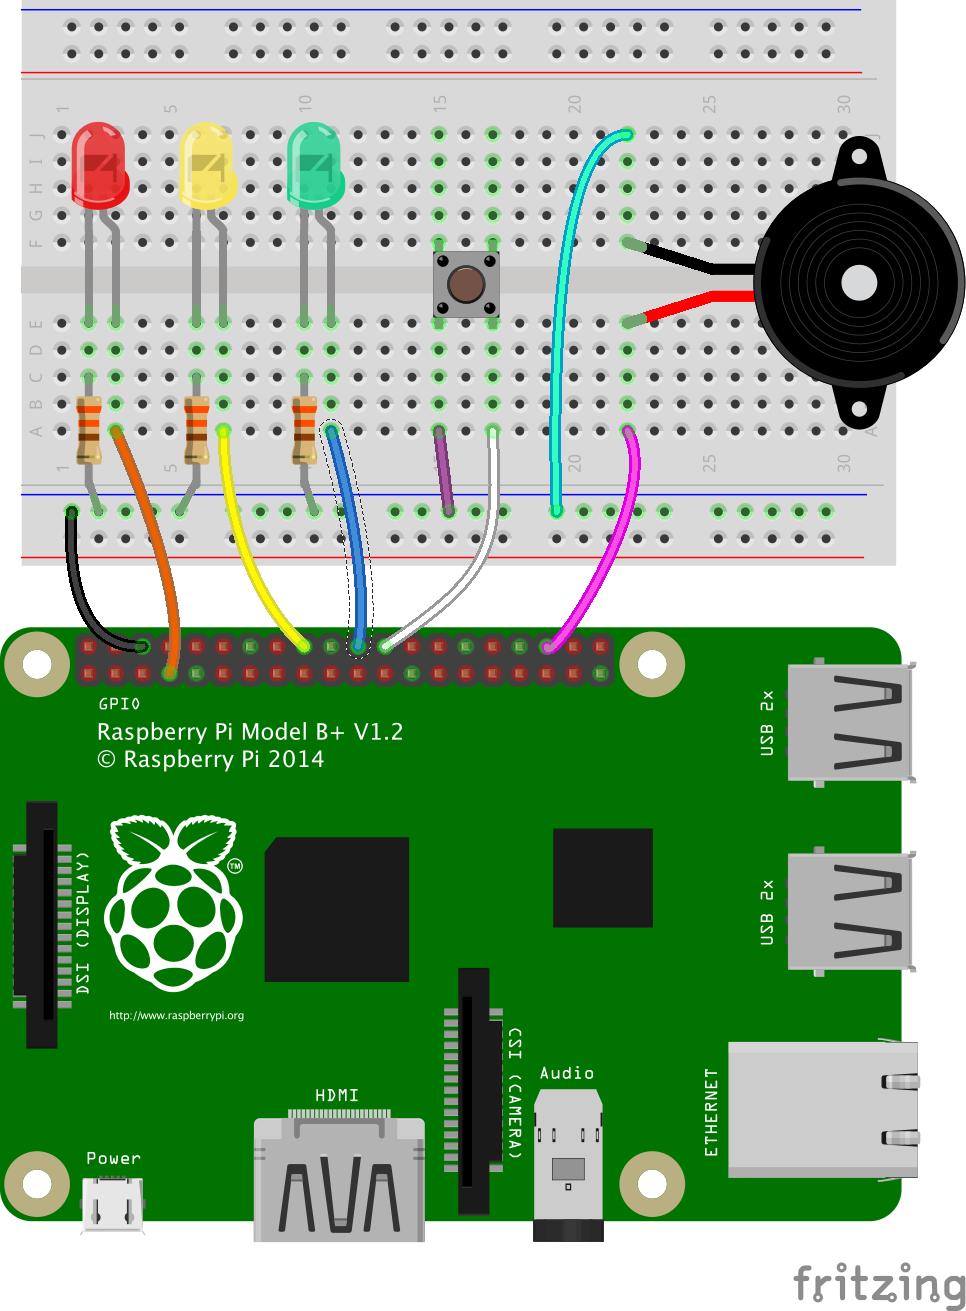
\includegraphics[width=0.75\textwidth]{buzzer-circuit}
\end{figure}

\subsection*{Exercise}

In this worksheet, you are going to program your Raspberry Pi with EduKit to act like a standard UK Pelican Crossing traffic light.  All UK lights work in the same way so that drivers know what to expect when they approach them.

Using the techniques learnt in the previous worksheets, your aim is to make the kit act like the traffic lights at a Pelican Crossing, reacting to the button press to allow pedestrians to cross.  The LEDs will act as signals to the vehicles; the buzzer will act as a signal to the pedestrians.

The standard sequence is as follows:
\begin{center}
\small
\begin{tabular}{|>{\centering\arraybackslash}p{0.24\textwidth}>{\centering\arraybackslash}p{0.24\textwidth}>{\centering\arraybackslash}p{0.24\textwidth}>{\centering\arraybackslash}p{0.16\textwidth}|}
\hline
\textbf{Action} & \textbf{Signal to Vehicles} & \textbf{Signal to Pedestrians} & \textbf{Timings} \\
\hline
 & Steady Green & Red Standing Figure & \\
\hline
Pedestrian presses the button & Steady Amber (Cars should stop if they can) & Red Standing Figure & 3 seconds \\
\hline
& Steady Red (Cars must stop) & Red Standing Figure & 1 second \\
\hline
Pedestrians can start walking & Steady Red & Green Walking Figure and Beeping & 4 to 7 seconds \\
\hline
Pedestrians should not start to cross & Steady Red & Flashing Green Figure and no sound & 2 seconds \\
\hline
& Flashing Amber (Cars can start to go again if the crossing is clear) & Flashing Green Figure & 6 seconds \\
\hline
& Flashing Amber & Red Standing Figure & 1 second \\
\hline
& Steady Green (Cars can proceed) & Red Standing Figure & At least 20 seconds \\
\hline
\end{tabular}
\end{center}

On the last step, the button can be pressed within the 20 seconds, but the lights should not change immediately.  After the 20 seconds, the process can start again.

Using knowledge from the previous CamJam worksheets, and the outline code, write your traffic light code!

\subsection*{Code Hints}

The `TI' variable gives the number of \emph{jiffies} since your computer was turned on.  A jiffy is $1/60$th of a second.  You can use it to time events or ensure that a certain amount of time has gone by.

Remember that `PEEK(UP) AND B' will extract just the bit referred to by B from the user port.  This can be used to see if that input has been triggered.  The input will be 0 if the action happened and B if no action happened.

\subsection*{Outline Code}

There are comments where you need to fill in some code.
\begin{basic}
10 REM TRAFFIC LIGHTS
20 REM SETUP LOCATIONS
30 UP=56577:DDR=56579
40 REM PIN VALUES FOR LEDS AND BUTTON
50 R=1:Y=2:G=4:B=8:Z=16:A=R+Y+G+Z
60 REM SET ONLY PINS 0,1,2, AND 4 FOR OUTPUT
70 POKE DDR,A
80 REM CLEAR USER PORT (ALL PINS OFF)
90 POKE UP,0
100 PRINT CHR\$(147);:REM CLEAR SCREEN
110 PRINT "TRAFFIC LIGHTS"
120 GOSUB 1100:REM INITIAL STATE
130 NP=B:REM BUTTON NOT PRESSED
140 S=TI:REM RECORD CURRENT TIME
150 FOR I=1 TO 72:NEXT I:REM 0.1 SECOND PAUSE
160 NP=PEEK(UP) AND B:REM CHECK IF NOT PRESSED
170 REM NP=0: PRESSED, NP=B: NOT PRESSED
180 IF NP=0 THEN GOSUB 1900:REM START SEQUENCE
190 IF NP<>0 THEN 150:REM LOOP WHILE NOT PRESSED
200 GOTO 130:REM LOOP FOREVER
1000 REM A DELAY OF D SECONDS
1010 T=D*720
1020 FOR I=1 TO T:NEXT I
1030 RETURN
1100 REM SETUP INITIAL STATE: GREEN ON, REST OFF
1102 REM PEDESTRIAN LIGHTS: RED ON, GREEN OFF
1190 RETURN
1200 REM GREEN OFF, AMBER ON FOR 3 SECONDS
1202 REM PEDESTRIAN LIGHTS: RED STILL ON
1290 RETURN
1300 REM AMBER OFF, RED ON FOR 1 SECOND
1302 REM PEDESTRIAN LIGHTS: RED STILL ON
1390 RETURN
1400 REM BUZZER FOR 4 SECONDS
1401 REM 0.5s ON, 0.5s OFF
1402 REM PEDESTRIAN LIGHTS: RED OFF, GREEN ON
1490 RETURN
1500 REM BUZZER OFF FOR 2 SECONDS
1502 REM PEDESTRIAN LIGHTS: GREEN FLASHING
1590 RETURN
1600 REM AMBER FLASHING FOR 6 SECONDS
1602 REM PEDESTRIAN LIGHTS: GREEN FLASHING
1690 RETURN
1700 REM AMBER FLASHING FOR 1 MORE SECOND
1702 REM PEDESTRIAN LIGHTS: GREEN OFF, RED ON
1790 RETURN
1800 REM TRAFFIC LIGHT SEQUENCE
1810 REM CALL SUBROUTINES IN CORRECT ORDER
1890 RETURN
1900 REM PREPARE TO START LIGHT SEQUENCE
1910 N=TI:REM CURRENT TIME
1920 REM KEEP CHECKING UNTIL 20 SECONDS REACHED
1930 IF (N-S)/60 <= 20 THEN 1910
1940 GOSUB 1800:REM RUN TRAFFIC LIGHT SEQUENCE
1950 RETURN
\end{basic}

Save your program as ``7 TRAFFIC LIGHTS''.

\subsection*{Running the Code}

Run the code.  If errors are reported, check your code again.  Press the button while the green LED is lit and see what happens.

\subsection*{Challenge}

Use a second CamJam EduKit, or additional red and green LEDs and 330$\Omega$ resistors, and use them as the Red and Green pedestrian figures.
